% theoretical overview

\def\sighat{\hat{\sigma}}

\section{Standard Model}
% http://pdg.lbl.gov/2013/reviews/rpp2012-rev-standard-model.pdf

All known interactions can be described by four fundamental forces. Listed in the increasing order of strength, they are: gravity, the weak nuclear force, electromagnetism, and the strong nuclear force. While Albert Einstein's general theory of relativity provides an excellent classical description of gravitational interactions on the macroscopic scales~\cite{GRcite}, a consistent quantum theory of gravity continues to elude theoretical physicists. However, in the domain of physics probed in this thesis, gravity is completely negligible, being 32 orders of magnitude smaller than the weak nuclear force.\footnote{In natural units, the ratio of forces corresponds to the ratio-squared of W boson mass (80 GeV) to Planck mass (1e18 GeV). This large discrepancy is better known as the ``hierarchy problem''.}

The remaining three forces can be interpreted in the quantum-theoretical framework of the Standard Model of particle physics (Fig.~\ref{fig:theory:SM}). A non-abelian gauge theory with the symmetry group $SU(3)$x$SU(2)$x$U(1)$, the Standard Model postulates that all matter is made of fermions (quarks and leptons), which are arranged into three generations separated by different flavor quantum numbers and masses. Interactions between fermions are mediated by the exchange of gauge bosons: $SU(3)$ generates gluons that carry the strong nuclear force, $SU(2)$ generates W bosons responsible for the weak charged currents, while the linear combination of neutral bosons from $SU(2)$ and $U(1)$ produces Z bosons, which mediate weak neutral currents, and photons, which mediate the electromagnetic force. Finally, a complex scalar field generates masses of elementary particles through the Higgs mechanism~\cite{PhysRevLett.13.508}.

This thesis focuses on the measurement of the production cross-section of \Wboson\ gauge bosons at the LHC. The mechanism of \Wboson\ production is explored in the next section.

\begin{figure}[phtb]
  \begin{center}
    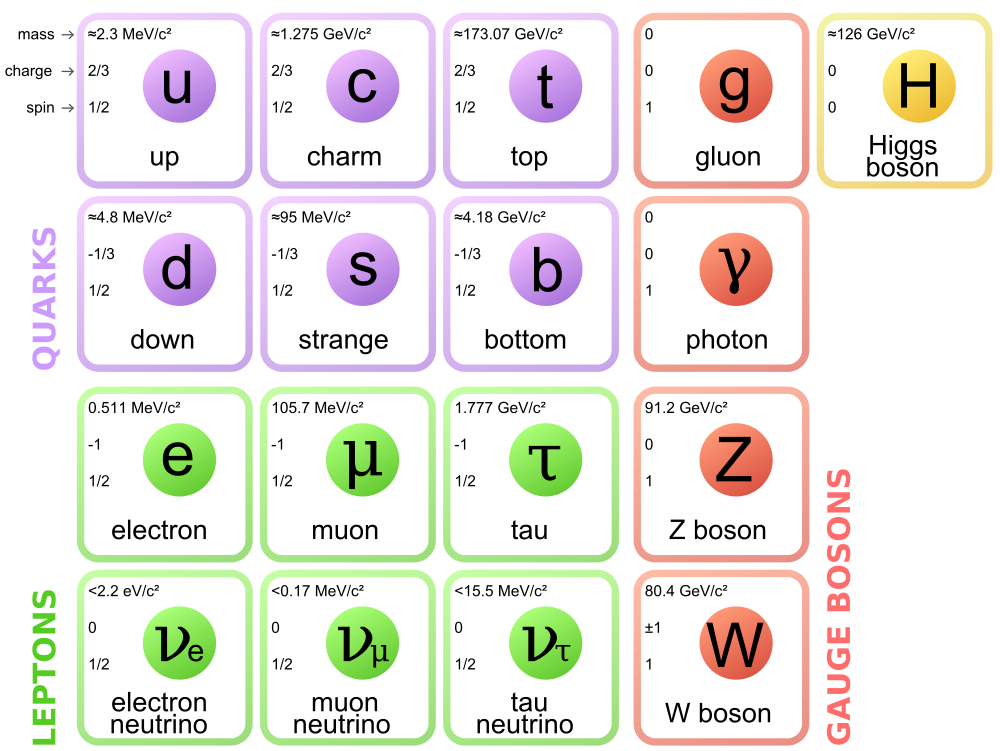
\includegraphics[width=0.7\textwidth]{theory/fig/SM}
    \caption{ The Standard Model of elementary particles.}
    \label{fig:theory:SM}
 \end{center}
\end{figure}

\section{ Hadron Scattering }
\label{chap:qcd_theory}

% Electroweak W gauge bosons are produced through proton-proton scattering at the LHC. 

In the first half of the 20th century, protons were considered to be point particles that, along with neutrons, combined to form the nuclei of all known atoms. Deep inelastic scattering experiments, which involve bombardment of protons by electrons, revealed non-trivial compositeness of the proton and led to the development of the parton model~\cite{PhysRevLett.23.1415}.

Under the parton model, protons consist of three valence quarks: two of up-type and one of down-type. These quarks spontaneously produce gluons, which in turn can split into additional quark-antiquark pairs, known as ``sea quarks''. Collectively, this swarm of constituents inside the proton are called partons. The fraction of the total proton momentum carried by each constituent is conventionally labeled ``x'', which varies from 0 to 1. Parton distribution functions (PDFs) are probability distributions of $x$ for different kinds of partons (see Sec.~\ref{chap:pdf_theory}).

According to the factorization theorem postulated by Drell and Yan~\cite{PhysRevLett.25.316}, a hard scattering collision between protons $A$ and $B$ can be viewed as an interaction between two free partons $a$ and $b$ with respective momentum fractions $x_a$ and $x_b$, weighted by the probability of carrying these momentum fractions (PDFs). The parton-parton interaction can be calculated in the context of perturbative quantum chromodynamics (QCD), amounting to a calculation of the relevant Feynman diagrams to a given order. The PDFs, however, are not calculable from the first principles and have to be determined experimentally. The key statement of the factorization theorem, illustrated in Fig.~\ref{fig:theory:hardscatter}, is that the PDFs are independent of the parton-parton process.

\begin{figure}[phtb]
  \begin{center}
    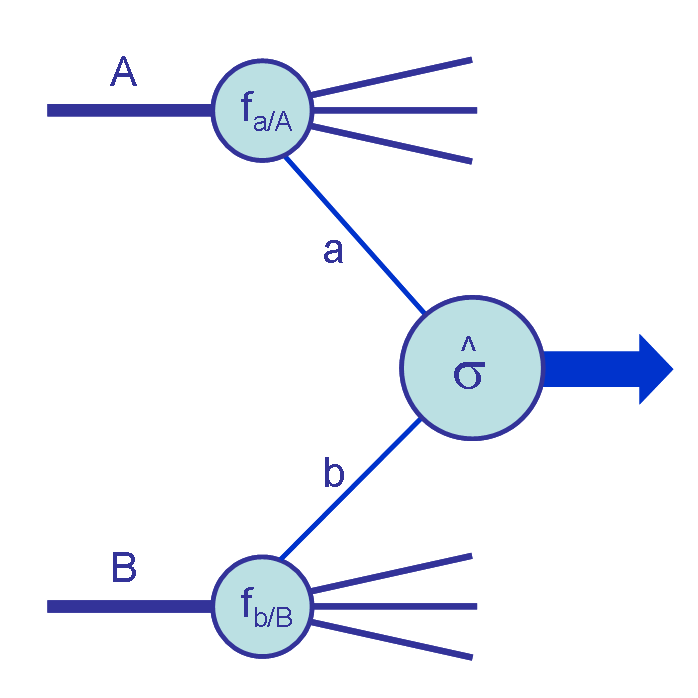
\includegraphics[width=0.4\textwidth]{theory/fig/Hardscattering}
    \caption{ Illustration of the factorization theorem in a hard-scattering process. $\sighat$ is the hard scattering cross-section, while small f's represent PDFs for each incoming proton. }
    \label{fig:theory:hardscatter}
 \end{center}
\end{figure}

Mathematically, the factorization theorem allows the cross-section of $AB\to W$ (where A,B are incoming protons) to be expressed by the following formula:
\begin{equation}
\begin{split}
\sigma_{AB\to W} = \sum\limits_{partons} \int dx_a dx_b\; f_{a/A}(x_a,\mu_{F}^2) f_{b/B}(x_b,\mu_{F}^2) \cdot \\
\left[ \sighat_{LO}(x_{a}x_{b}s) + \alpha_{s}(\mu_{R}^2)\sighat_{NLO}(x_{a}x_{b}s) + \left(\alpha_{s}(\mu_{R}^2)\right)^{2}\sighat{NNLO}(x_{a}x_{b}s) + \ldots \right]
\end{split}
\label{sigll}
\end{equation}
The meaning of all variables is explained below.

The partonic cross-section $\sighat$ is expanded in powers of the strong interaction coupling constant $\alpha_{s}$, where higher-order perturbation terms correspond to Feynman diagrams with additional emissions. The cross-section at each order depends on the energy scale $Q^2 \equiv x_{a}x_{b}s$, where $\sqrt s$ is the center-of-mass energy of proton collisions. $\alpha_{s}$ depends on a non-physical parameter $\mu_{R}$ - the renormalization scale of the QCD running coupling. Intuitively, renormalization avoids ultraviolet infinities in higher-loop diagrams by re-defining the coupling constant when probing the interaction at different energy scales. The PDFs $f_{a/A}(x_a,\mu_{F}^2)$\footnote{$f_{a/A}$ refers to a parton $a$ from the incoming hadron $A$} and $f_{b/B}(x_b,\mu_{F}^2)$ depend on another non-physical parameter $\mu_{F}$, known as the factorization scale. This is the energy scale that separates perturbative and non-perturbative pieces of the calculation, with the latter being absorbed into the definition of the PDF. These non-perturbative elements correspond to soft collinear gluon emissions, which produce infrared singularities in the perturbation theory.

In principle, the numerical cross-section is independent of the renormalization and factorization scales, with all non-physical dependencies canceling out if the series expansion is carried to all orders of $\alpha_{s}$. However, because practical considerations require that the calculation is stopped early (usually at NLO or NNLO), some dependence of the cross-section on these non-physical parameters is retained. The conventional prescription is to choose $\mu_{R}$ and $\mu_{F}$ to be of the same order as the typical momentum transfer in the hard scattering process. More specifically, $\mu_{R}$ and $\mu_{F}$ are both set to the mass of the produced \Wboson\ boson, but are allowed to vary by a factor of 2 of their central values, resulting in additional theoretical uncertainty on the cross-section.

\subsection{W production}

The leading-order diagram for \Wboson\ production is shown in Fig.~\ref{fig:theory:feynlo}.

\begin{figure}[phtb]
  \begin{center}
    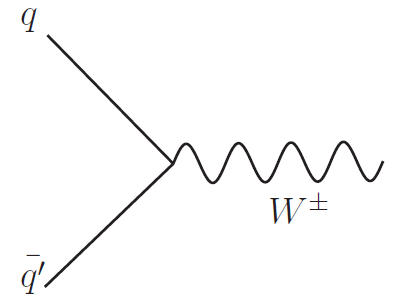
\includegraphics[width=0.3\textwidth]{theory/fig/feynlo}
    \caption{ Leading-order diagram of \Wboson\ production through quark-antiquark annihilation.}
    \label{fig:theory:feynlo}
 \end{center}
\end{figure}

The cross-section $\sighat$ of this diagram can be calculated with standard quantum field theory techniques and yields~\cite{PDG}:
$$ \sighat(q\bar{q'} \rightarrow W) = 2\pi|V_{qq'}|^2 \frac{G_F}{\sqrt{2}} M_{W}^{2} \cdot \delta\left(Q^2 - M_{W}^{2}\right)$$
where $G_F$ is the Fermi coupling constant, $|V_{qq'}|$ is the relevant element from the Cabibbo-Kobayashi-Maskawa (CKM) quark mixing matrix~\cite{Kobayashi01021973}, $M_W$ is the mass of the W boson, and $\delta$ is the Dirac delta function. Beyond leading order, the relationship becomes more complex, and the restriction on $Q^2=M_{W}^{2}$ is relaxed.

Fig.~\ref{fig:theory:Wprod} shows that the dominant production channel for $W^+$ is through $u\bar{d}$, where the up quark is a valence quark while the anti-down comes from the sea (and similarly for $W^-$ with $\bar{u}d$). At 7 TeV, about 10\% of \Wboson\ bosons are produced through strange-charm annihilation, followed by a negligible contribution from CKM-suppressed cross-family processes.

\begin{figure}[phtb]
  \begin{center}
    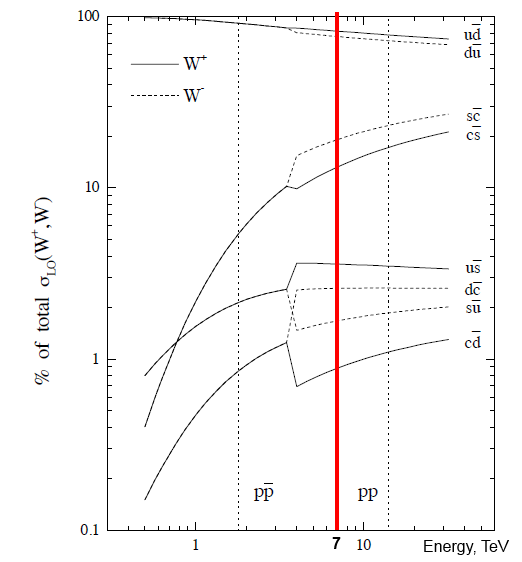
\includegraphics[width=0.55\textwidth]{theory/fig/Wprod}
    \caption{ Contributions of several quark-antiquark processes to \Wboson\ production cross-section. The red line marks the collision energy relevant to this analysis (7 TeV). }
    \label{fig:theory:Wprod}
 \end{center}
\end{figure}

\subsection{Parton Distribution Functions}
\label{chap:pdf_theory}

Parton distribution functions quantify the probability distributions of the momentum fraction $x$ for partons within a hadron. They are not calculable from first principles in perturbation theory and have to be determined experimentally through a global fit to various experimental data~\cite{pdfmaster}. Because experiments may operate at different energy transfer points, the PDFs are extrapolated to a common energy scale $Q^2$ in fits to experimental data, which is accomplished through the so-called DGLAP evolution equations~\cite{Dokshitzer:1977sg,Gribov:1972ri,Altarelli:1977zs}. Similar to scattering amplitude calculations, PDFs can be defined at different orders of perturbation theory.

By way of introduction, suppose $u(x)$ and $d(x)$ are PDFs for up and down quarks, while $\bar{u}(x)$ and $\bar{d}(x)$ are PDFs of the corresponding anti-quarks. In a proton, valence quarks are identified as $u_v=u-{\bar u}$ and $d_v=d-{\bar d}$, which implies the following constraints on the proton PDFs~\cite{0034-4885-76-4-046201}:
\begin{eqnarray}
\int_0^1 \left[u(x)-\bar{u}(x) \right] \, {\rm d}x = 2   \hspace{2cm}  
\int_0^1 \left[d(x)-\bar{d}(x) \right] \, {\rm d}x = 1 \,\,\,   \label{eq:countingrule} \\
{\rm{and}} \hspace{1cm} \int_0^1 \left[q(x)-\bar{q}(x) \right] \, {\rm d}x = 0 \hspace{1cm} {\rm{for }} \quad q=s,c,b,t
\label{eq:countingrule2}
\end{eqnarray}

Fig.~\ref{fig:example_pdfs} shows an example of proton PDFs from the CT10 collaboration~\cite{Lai:2010vv} at two different $Q^2$ scales. From the PDF curves, one sees that (1) valence quarks tend to carry a much higher fraction of proton momentum, and (2) gluon and sea quark distributions increase dramatically at higher energy scales.

\begin{figure}[htb]
\begin{center}
\begin{tabular}{cc}
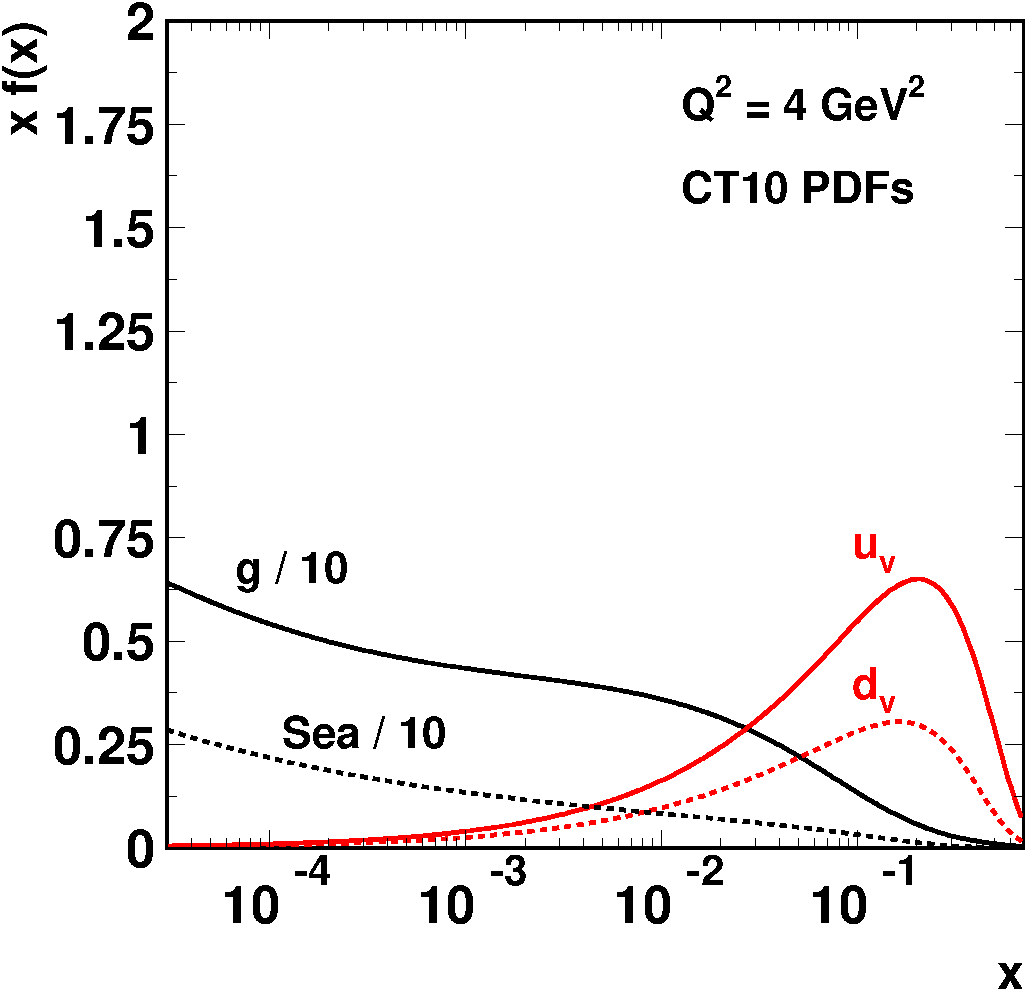
\includegraphics[width=0.45\columnwidth]{theory/fig/examplepdfs_q2} &
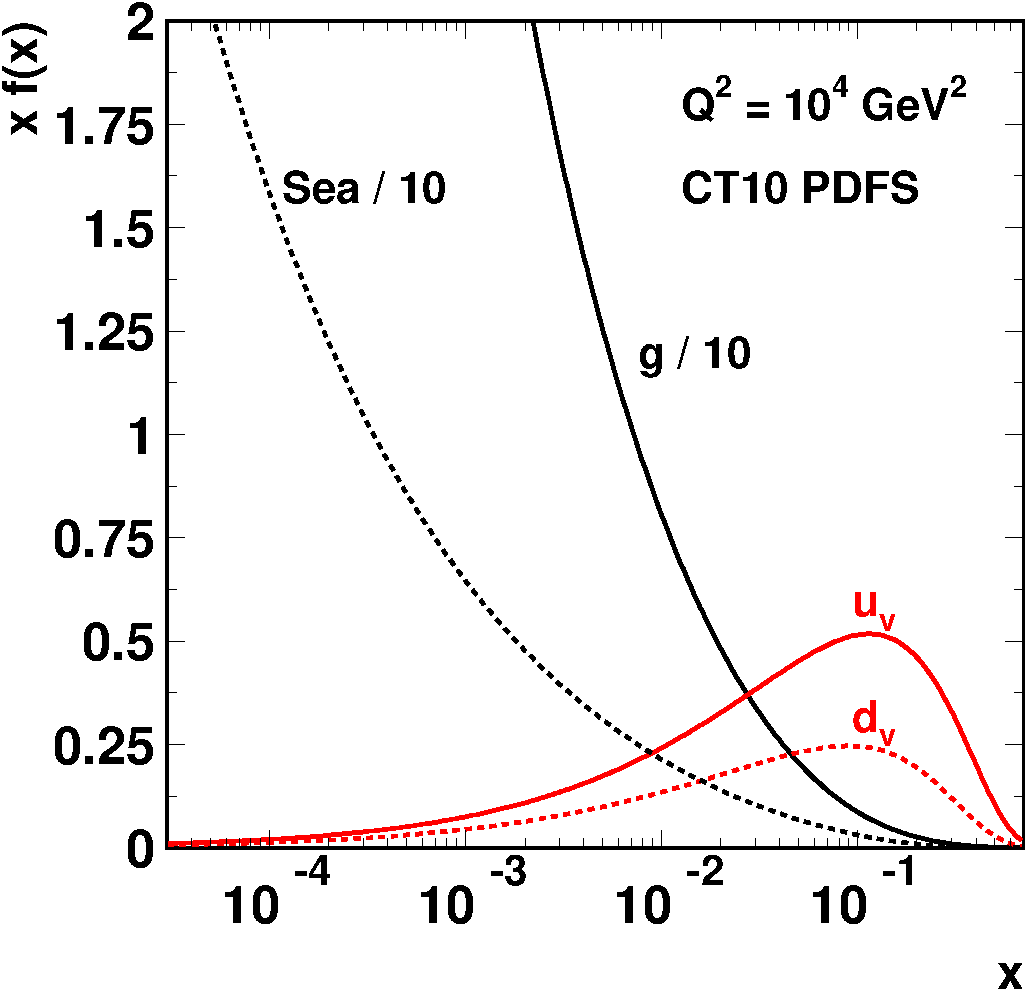
\includegraphics[width=0.45\columnwidth]{theory/fig/examplepdfs_q100}
\end{tabular}
\end{center}
\caption{ Example PDFs at $Q^2 = 4$~GeV$^2$ and $Q^2 = 10^4$~GeV$^2$ (CT10 collaboration). }
\label{fig:example_pdfs}
\end{figure}

PDFs always come with an uncertainty band, which was not shown in Fig.~\ref{fig:example_pdfs}. This uncertainty is driven by experimental uncertainties in the input data and may be amplified by DGLAP evolution to a common energy scale $Q^2$. PDF uncertainties often play an important role in searches for new physics and precision measurements at collider experiments, so a lot of work has gone into developing robust PDF families~\cite{Alekhin:2012ig,Aaron:2009aa,Radescu:2011cn,Martin:2009iq,Ball:2012cx}. Global PDF fits can greatly benefit from new data inputs, particularly in sparsely studied regions of phase space. For example, Fig.~\ref{fig:theory:WZ_str_pdf_ratio} shows the effect of 2010 and 2011 W/Z inclusive cross-section measurements (this thesis is part of the latter) on the strange quark PDF uncertainty bands.

\begin{figure}[phtb]
  \begin{center}
    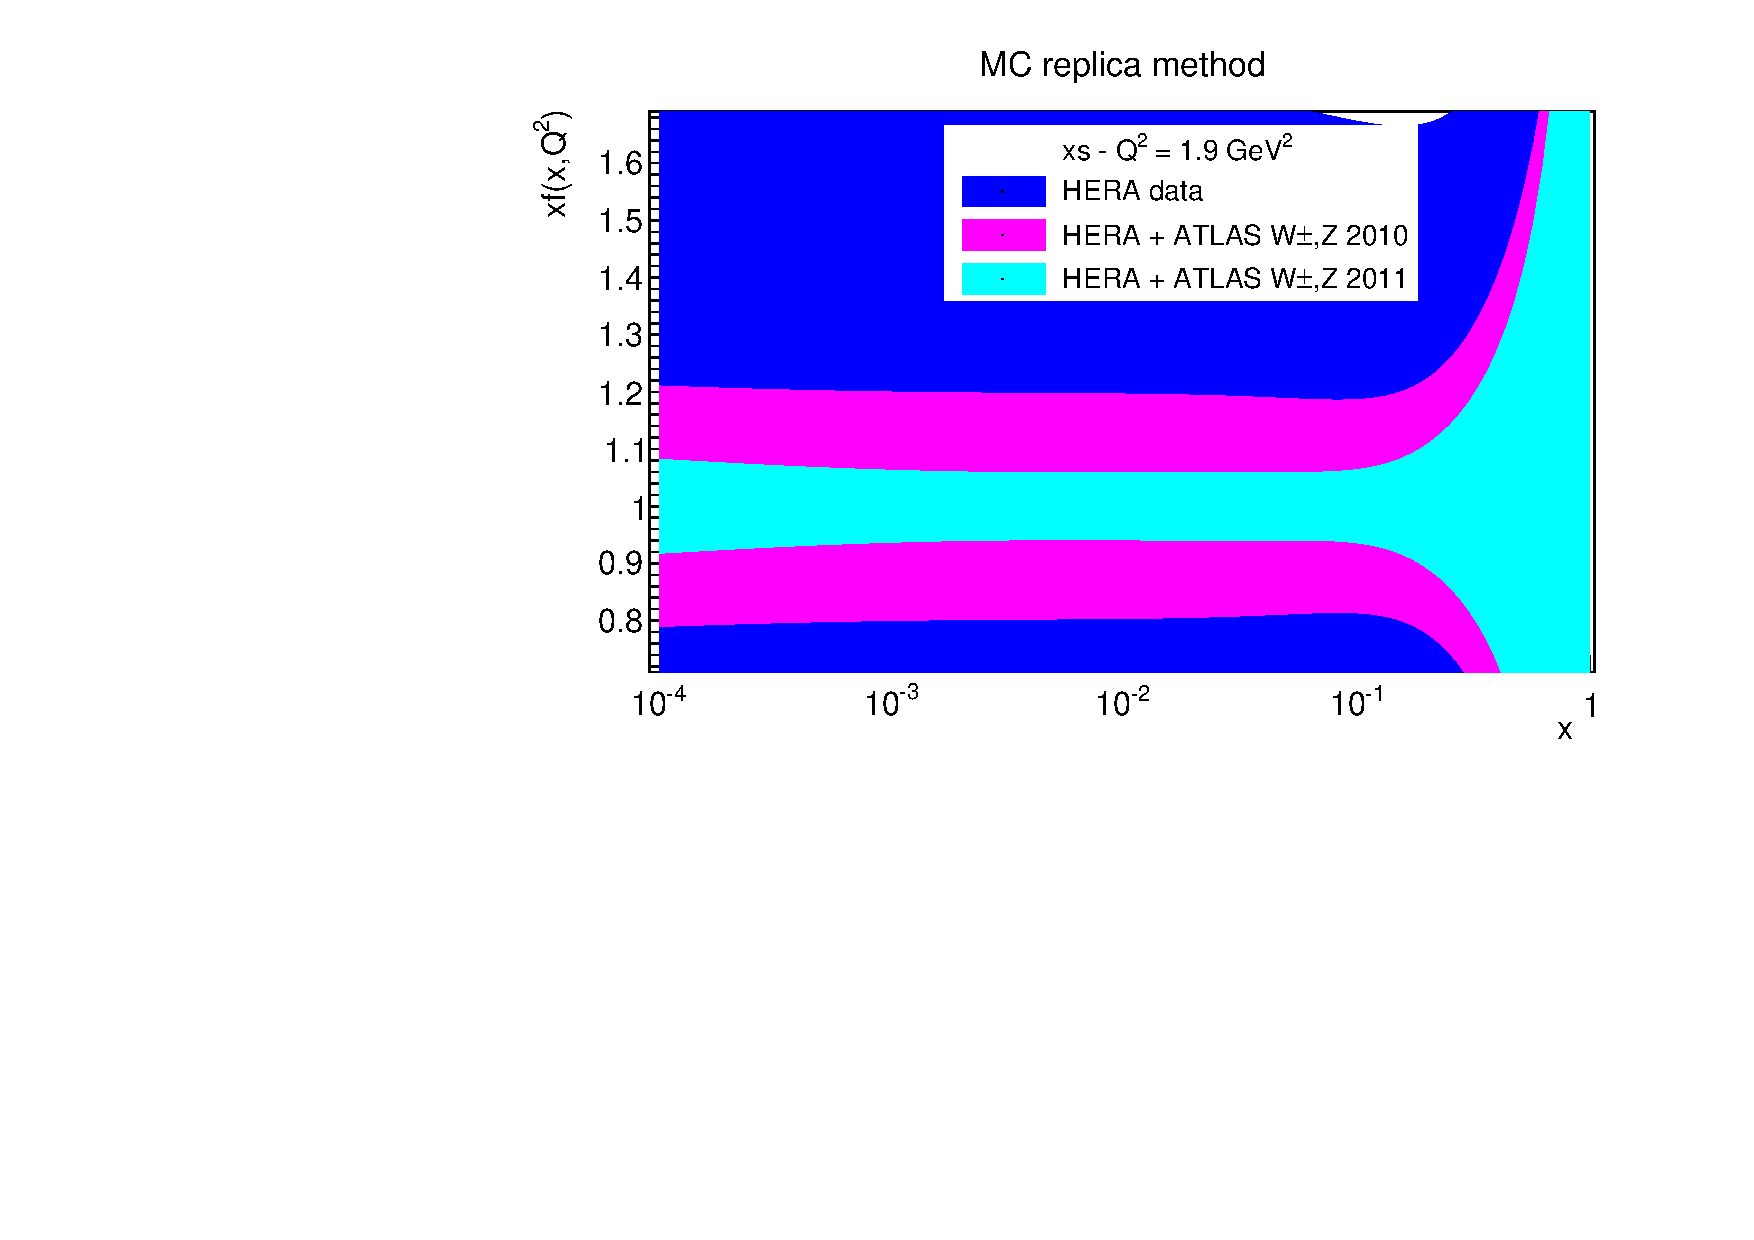
\includegraphics[width=0.7\textwidth]{theory/fig/WZ_str_pdf_ratio}
    \caption{ Strange quark PDFs using deep inelastic scattering data (HERA) alone, with the 2010 W/Z measurement, and with the 2011 W/Z measurement. Shaded regions represent 68\% confidence bands.}
    \label{fig:theory:WZ_str_pdf_ratio}
 \end{center}
\end{figure}

PDF coverage of different experiments is shown in Fig.~\ref{fig:theory:atlas_xq}. The high-$x$, low-$Q^2$ region is dominated by the fixed target experiments. A large region of phase space is covered by deep inelastic scattering data (for example, the solid orange HERA H1 curve). Higher $Q^2$ regions are best constrained by the hadron collider experiments. The measurement performed in this thesis provides the strongest sensitivity at $Q^2=M_{W}^2=80.4^2 GeV^2$ and $0.001<x<0.1$.

\begin{figure}[phtb]
  \begin{center}
    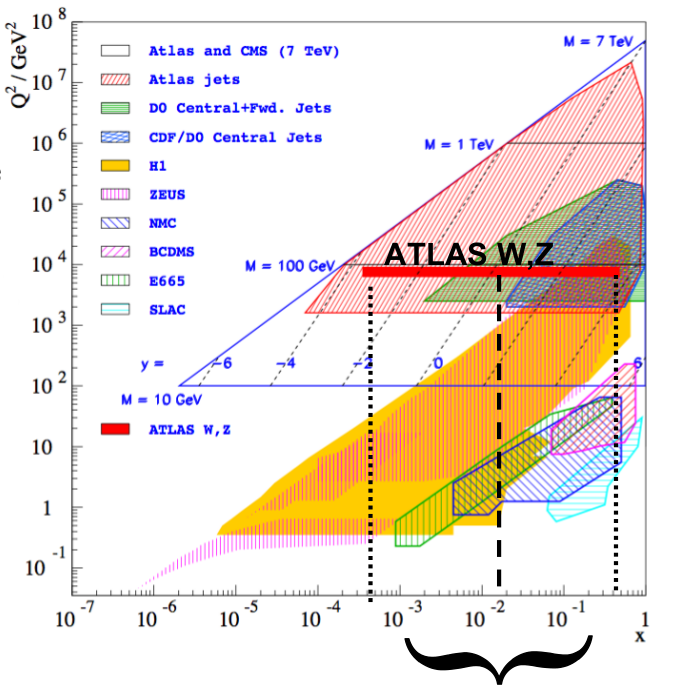
\includegraphics[width=0.5\textwidth]{theory/fig/atlas_xq}
    \caption{ Sensitivity region of various experimental inputs in constraining PDFs.}
    \label{fig:theory:atlas_xq}
 \end{center}
\end{figure}

\subsection{ PDFs and W rapidity }
\label{sec:theory:pdfrap}
Proton structure can be probed in a \Wboson\ cross-section measurement by looking at the boson rapidity $y$, defined as the boost along the beam axis from the lab frame to the frame where the boson moves only perpendicularly to the beam. Note that the pseudorapidity $\eta$ is equal to rapidity $y$ in the limit where $E \gg m$, where $E$ is energy and $m$ is mass.

Boson rapidity is related to parton momentum fractions $x_a$ and $x_b$ through the following relationship:
\begin{equation}
y_W \equiv \frac{1}{2} \cdot ln \left( \frac{E + p_z}{E - p_z} \right) = \frac{1}{2} \cdot ln \left( \frac{x_a}{x_b}\right)
\label{theory:rapidity}
\end{equation}

Setting $Q^2 = m_W^2$ and using the fact that $Q^2 = x_{a}x_{b}s$, we arrive at a direct relationship between the boson rapidity and PDF momentum fractions of the quark-antiquark pair that annihilate to produce the \Wboson\ boson:
$$ x_a = \frac{m_W}{\sqrt s} e^{y_W} $$
$$ x_b = \frac{m_W}{\sqrt s} e^{-y_W} $$

Intuitively, the relationship makes sense: if $x_a$ is substantially higher than $x_b$, the parton coming from proton A will carry a greater momentum and the \Wboson\ boson will be produced moving along the beam axis, which is an intuitive proxy for the boson rapidity.

\section{W Decay and Muon Pseudorapidity}

Fig.~\ref{fig:theory:decay} shows the decay channel studied in this thesis: \Wmn.

\begin{figure}[phtb]
  \begin{center}
    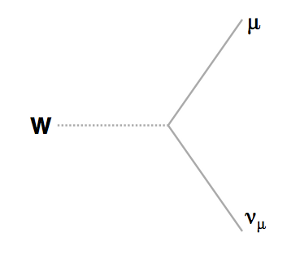
\includegraphics[width=0.25\textwidth]{theory/fig/decay}
    \caption{ Decay of the \Wboson\ boson into a muon and a neutrino.}
    \label{fig:theory:decay}
 \end{center}
\end{figure}

Reconstructing boson rapidity requires information about all three components of the muon and neutrino momenta. However, the $p_z$ component of the neutrino is inaccessible experimentally: only the transverse component $p_T$ is measured through the missing transverse energy. As a result, measurement of the \Wboson\ rapidity requires imposition of a \Wboson\ mass constraint, which produces a quadratic equation for the missing longitudinal component of neutrino momentum. The ambiguity in selecting the correct solution of that quadratic equation renders boson rapidity undesirable in studying the proton structure.

\begin{figure}[phtb]
  \begin{center}
    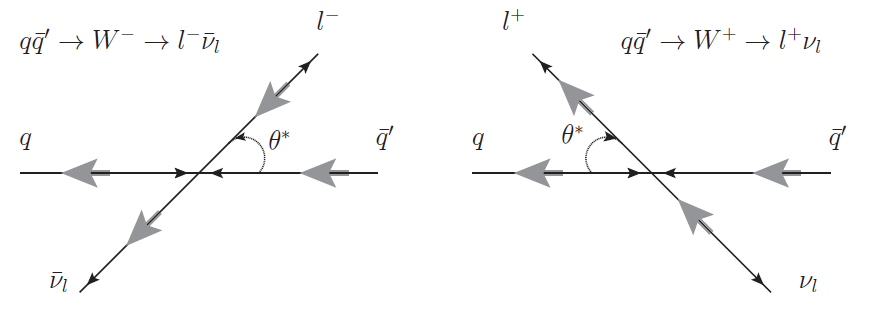
\includegraphics[width=0.7\textwidth]{theory/fig/VA}
    \caption{ Decay diagrams in the rest frame of the \Wboson. Black arrows show the direction of motion; gray arrows indicate the spin. The \Wboson\ spin always points in the direction of the incoming anti-quark.}
    \label{fig:theory:va}
 \end{center}
\end{figure}

A good alternative is to measure the pseudorapidity $\eta$ of the muon, which does not require any knowledge about neutrino $p_z$. The vector minus axial-vector (V-A) nature of the \Wboson\ decay preserves the correlation between boson rapidity $y_W$ and muon pseudorapidity $\eta_\mu$~\cite{MartinezOutschoorn:2011hta}. Fig.~\ref{fig:theory:va} shows preferred decay orientations in terms of $\theta^*$, the angle between the muon in the \Wboson\ rest frame and the direction of the \Wboson, which is distributed according to:
$$ \frac{dN}{d \cos(\theta^*)} = \left(1 \pm \cos(\theta^*) \right)^{2}$$
The sign depends on the product of the W and muon helicities.

As a result, it is possible to deduce information about parton momentum fractions from the pseudorapidity distribution by de-convolving the known V-A correlation between the boson rapidity and the muon pseudorapidity.

\section{Parton Shower and Hadronization}

In addition to the physics of hard collisions outlined above, several additional effects must be considered to fully understand an event at the hadron collider (Fig.~\ref{fig:theory:ps}).

Particles leaving the hard scattering vertex are able to radiate additional particles, which must be taken into account by Monte-Carlo programs. This process is called parton showering (PS), and several variations exist differing in the exact treatment of additional emissions (for example, angular-ordered or virtuality-ordered).

Hadronization is the process by which particles carrying color, which cannot exist in free form, recombine into colorless duplets or triplets. As with parton showering, several implementations are available in Monte-Carlo programs, such as the string or cluster model.

\begin{figure}[phtb]
  \begin{center}
    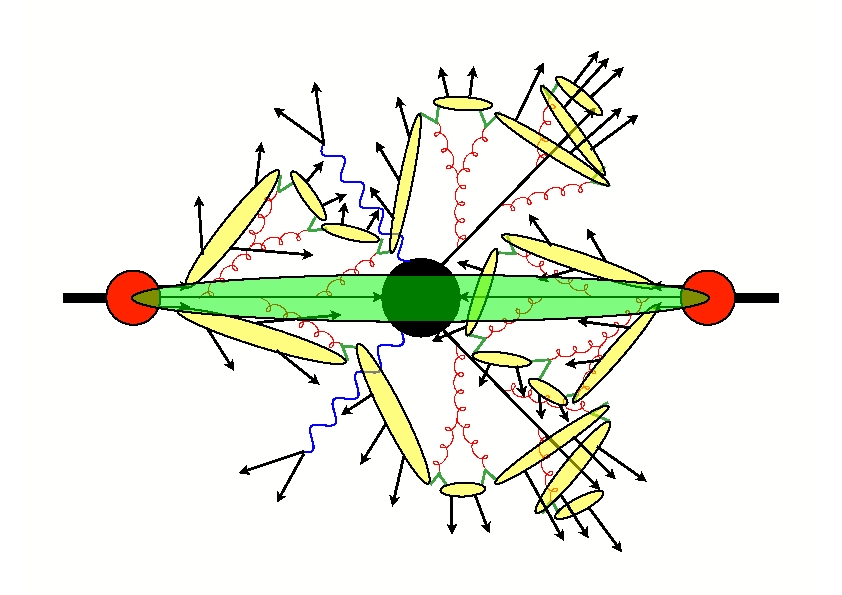
\includegraphics[width=0.55\textwidth]{theory/fig/ps}
    \caption{ A diagram depicting parton showering (additional emissions) and hadronization (formation of colorless hadrons represented as yellow blobs). The original hard process is shown as a black blob in the middle of the picture.}
    \label{fig:theory:ps}
 \end{center}
\end{figure}

\section{Theoretical Predictions}
\label{sec:theory:nnlo}
This section outlines the practical aspects of theoretical predictions used in this analysis. Computationally intensive and requiring careful fine-tuning of the Monte-Carlo programs, these calculations demanded a considerable effort by a dedicated theory team.

Theoretical predictions of hadronic W and Z production cross-sections were calculated to NLO and NNLO QCD using the programs
FEWZ~\cite{Gavin:2010az, Gavin:2012sy, Li:2012wn} and
DYNNLO~\cite{Catani:2007vq,Catani:2009sm}.
These are the only available programs that allow the computation of
NNLO cross-section while applying fiducial kinematic cuts.

The following NNLO PDF families were interfaced with FEWZ and DYNNLO:
\begin{itemize}
\item CT10 NNLO~\cite{Lai:2010vv},
\item ABM11 NNLO~\cite{Alekhin:2012ig},
\item HERAPDF 1.5 NNLO~\cite{Aaron:2009aa,Radescu:2011cn},
\item MSTW2008 NNLO~\cite{Martin:2009iq},
\item NNPDF2.3 NNLO $\alpha_S = 0.118$~\cite{Ball:2012cx}, and
\item JR09 NNLO~\cite{JimenezDelgado:2008hf}.
\end{itemize}

Electroweak parameters were chosen according to the Particle Data Group recommendations~\cite{PDG} and listed in Tab.~\ref{tab:EW parameters}.

\begin{table}[tb]
  \begin{center}
\begin{tabular}{lrlr}
\hline
\hline
    $M_Z$                       & 91.1876 GeV                        & $V_{ud}$      & 0.97427  \\
    $\Gamma_Z$                  & 2.4949 GeV                            & $V_{us}$      & 0.22534  \\
    $\Gamma(Z \rightarrow ll)$  & 0.084 GeV                             & $V_{ub}$      & 0.00351  \\
    $M_W$                       & 80.385 GeV                        & $V_{cd}$      & 0.22520  \\
    $\Gamma_W$                  & 2.0906 GeV                            & $V_{cs}$      & 0.97344  \\
    $\Gamma(W \rightarrow l\nu)$ & 0.22727 GeV                          & $V_{cb}$      & 0.0412   \\
    $M_H$                       & 125     GeV                        & $V_{td}$      & 0.00867  \\
    $m_t$                       & 173.5   GeV                        & $V_{ts}$      & 0.0404   \\
    $G_F$                       & $1.166 \times 10^{-5}$ GeV$^{-2}$ & $V_{tb}$      & 0.999146 \\
    $sin^2\theta_W$             & 0.2229                   &               &       \\
    $\alpha_G$                  & $7.5624 \times 10^{-3}$  &               &       \\
    $vec_{up}$                  & 0.4056                   &               &       \\
    $vec_{dn}$                  & -0.7028                  &               &       \\
    $vec_{le}$                  & -0.1084                  &               &       \\

    \hline
    \hline
    \end{tabular}
    \caption{Electroweak input parameters for evaluation of the $W^-$, $W^+$ and $Z$ cross-sections.}
    \label{tab:EW parameters}
  \end{center}
\end{table}
